\documentclass[12pt]{llncs}
\usepackage{tikz}
\usepackage{float}

\usetikzlibrary{calc}

\usepackage[
	backend=bibtex,
	style=numeric,
	sorting=none]{biblatex}
\addbibresource{references.bib}

\title{Modeling SARS-CoV-2 pandemic in NetLogo}
\author{Lorenzo Vainigli \\
lorenzo.vainigli@studio.unibo.it \\
matr. 0000842756}
\institute{Course of Complex Systems and Network Science \\
Laurea Magistrale in Informatica \\
University of Bologna \\
A.Y. 2020-2021}
\date{\today}

\pagestyle{plain}

\begin{document}
\maketitle

\begin{abstract}
This is the paper's abstract \ldots
\end{abstract}

\section{Introduction}

\section{Previous work}\label{previous work}
In the literature there is some works that I used to plan this project. The concepts of model that I used derived from a book written by Brauer et al., that shows the models that can be used in a simulation of virus spreading in a population \cite{brauer}. An article from Giordano et al. explain how to model the intervetions in the population to fight the COVID-19 outbreak \cite{giordano}, but it's too complex for the purposes of this project.\\
The Netlogo \cite{netlogo} models library offers a program that simulate the virus spreading in a population \cite{netlogo-virus}, it's very simple and general-purpose, but it was a good point to start the building of the model of this project.

\section{Studying}
In this section I will explain the process of thinking which models are better to use for the aim of the project and how I modified the ones from \cite{brauer}.

\subsection{Achievements}
The final achievement of this project is to build and study a network model that simulates the outbreak of the new SARS-CoV-2 virus. To do that, we must consider a situation in which we have a crowd of people that have contacts with each other, where there are some infected individuals that cause the spreading of the infection. Also some kind of quarantine and isolations are needed for who become infected. \\
We need a model similar to the SEIQJR model. Let's start from the simplest model, the SIS, and then add new classes to make a more complex model.

\subsection{The SIS model}
The SIS model is the simplest model in which there is a class of susceptible people ($S$) that, if one get the infection, goes to the infected class ($I$). Then, when infected people get recovered they returned to the susceptible class.

\paragraph{New classes}
\begin{itemize}
\item $S$ = Susceptible
\item $I$ = Infected
\end{itemize}

\paragraph{New variables}
\begin{itemize}
\item $a$ = infection rate;
\item $b$ = probability that an infected person get recovered.
\end{itemize}

\begin{figure}[H]
	\centering
    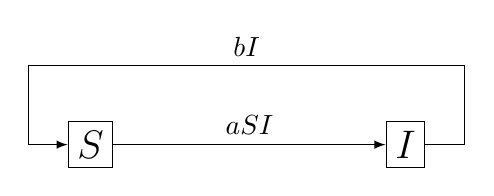
\begin{tikzpicture}
    \node[draw] at (0,0) (S) {\Large $S$};
    \node[draw] at (4,0) (I) {\Large $I$};
    \draw[draw, -latex] (S.east) -- (I.west) node [midway,above] {$aSI$};;
    \draw[draw, -latex] (I.east) -| ($(I.east)+(0.5,1)$) -- ($(S.west)+(-0.5,1)$) node [midway,above] {$bI$} |- (S.west);
    \end{tikzpicture}
    \caption{Diagram of the SIS model}
\end{figure}

$$\frac{dS}{dt} = -aSI + bI$$
$$\frac{dI}{dt} = aSI - bI$$

\subsection{The SEIS model}
As we know, SARS-CoV-2 infection leads an incubation period during which the infected person don't have symptoms but can transmit the infection to other people. We introduce an exposed class $E$ in which we put people that had have a contact with infected people and may be infected in an asymptomatic status.

\paragraph{New classes}
\begin{itemize}
\item $E$ = Exposed
\end{itemize}

\paragraph{New variables}
\begin{itemize}
\item $k$ = probability that exposed people become infective.
\end{itemize}

\begin{figure}
	\centering
    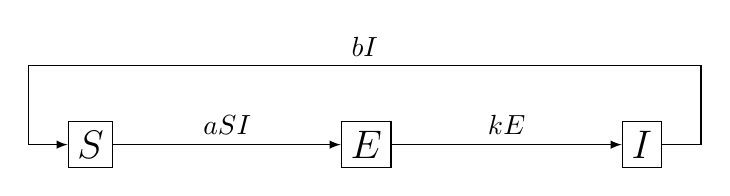
\begin{tikzpicture}
    \node[draw] at (0,0) (S) {\Large $S$};
    \node[draw] at (3.5,0) (E) {\Large $E$};
    \node[draw] at (7,0) (I) {\Large $I$};
    \draw[draw, -latex] (S.east) -- (E.west) node [midway,above] {$aSI$};
    \draw[draw, -latex] (E.east) -- (I.west) node [midway,above] {$kE$};
    \draw[draw, -latex] (I.east) -| ($(I.east)+(0.5,1)$) -- ($(S.west)+(-0.5,1)$) node [midway,above] {$bI$} |- (S.west);
    \end{tikzpicture}
    \caption{Diagram of the SEIS model}
\end{figure}

$$\frac{dS}{dt} = -aSI + bI$$
$$\frac{dE}{dt} = aSI - kE$$
$$\frac{dI}{dt} = kE - bI$$

\paragraph{\textbf{No immunity provided}}
Beacuse of the unknown properties of immunity from SARS-CoV-2, we can assume that the S class and R class coincide, creating a cycle that causes the comeback of the recoverd individuals in the susceptible class.

\subsection{The SEIQJS model}
Due to the unavailability of a vaccine, to fight SARS-CoV-2 infected people are quarantined or isolated (or, also, hospitalized). As suggested from the SEIQJR model, two classes were added: $Q$ is the class of quarantined people, i.e. the exposed people belong to the class $E$; $J$ is the class for isolate infected people of class $I$. So basically $Q$ is for $E$ what $J$ is for $I$, with the only difference that there is a flow from $Q$ to $J$ but not vice versa.\\
People isolated (i.e. belong to class $J$) can recover as people belong to class $I$.

\paragraph{New classes}
\begin{itemize}
\item $Q$ = Quarantined
\item $J$ = Isolated
\end{itemize}

\paragraph{New variables}
\begin{itemize}
\item $\varepsilon_E$ = probability that a person exposed (in $E$) transmit the infection, exposed-transmission-factor;
\item $\varepsilon_Q$ = probability that a person quarantined (in $Q$) make a contact, quarantined-contact-factor;
\item $\varepsilon_J$ = probability that a person isolated (in $J$) transmit the infection, isolation-transmission-factor;
\item $k_E$ = probability that exposed people become infective;
\item $k_Q$ = probability that quarantined people are isolated;
\item $c_Q$ = percentage of exposed people that are quarantined at each time step;
\item $c_J$ = percentage of infected people that are isolated at each time step;
\item $b_I$ = probability that an infected person get recovered;
\item $b_J$ = probability that an isolated person get recovered;
\end{itemize}

\begin{figure}[H]
	\centering
    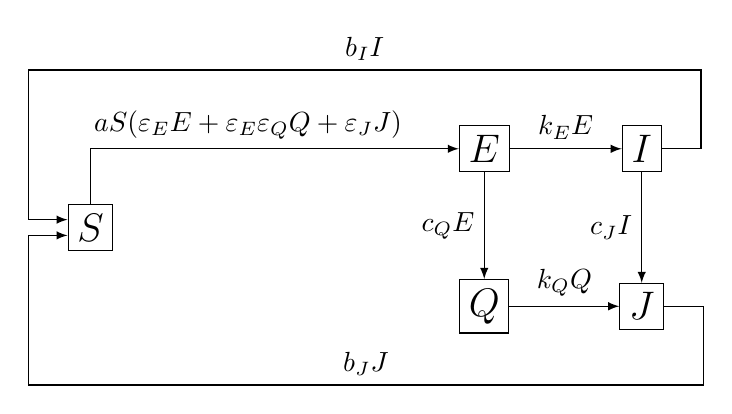
\begin{tikzpicture}
    \node[draw] at (0,0) (S) {\Large $S$};
    \node[draw] at (5,1) (E) {\Large $E$};
    \node[draw] at (5,-1) (Q) {\Large $Q$};
    \node[draw] at (7,1) (I) {\Large $I$};
    \node[draw] at (7,-1) (J) {\Large $J$};
    \draw[draw, -latex] (S.north) |- (E.west) node [midway,xshift=2cm,above] {$aS(\varepsilon_EE + \varepsilon_E\varepsilon_QQ + \varepsilon_JJ)$};
    \draw[draw, -latex] (E.south) -- (Q.north) node [midway,left] {$c_QE$};
    \draw[draw, -latex] (E.east) -- (I.west) node [midway,above] {$k_EE$};
    \draw[draw, -latex] (I.south) -- (J.north) node [midway,left] {$c_JI$};
    \draw[draw, -latex] (Q.east) -- (J.west) node [midway,above] {$k_QQ$};
    \draw[draw, -latex] (I.east) -| ($(I.east)+(0.5,1)$) -- ($(S.west)+(-0.5,2)$) node [midway,above] {$b_II$} |- ($(S.west)+(0,0.1)$);
    \draw[draw, -latex] (J.east) -| ($(J.east)+(0.5,-1)$) -- ($(S.west)-(0.5,2)$) node [midway,above] {$b_JJ$} |- ($(S.west)-(0,0.1)$);
    \end{tikzpicture}
    \caption{Diagram of the SEIQJS model}
\end{figure}

$$\frac{dS}{dt} = -aS(\varepsilon_EE + \varepsilon_E\varepsilon_QQ + \varepsilon_JJ) + b_II + b_JJ$$
$$\frac{dE}{dt} = aS(\varepsilon_EE + \varepsilon_E\varepsilon_QQ + \varepsilon_JJ) - (k_E + c_Q)E$$
$$\frac{dQ}{dt} = c_QE - k_QQ$$
$$\frac{dI}{dt} = k_EE - (b_I + c_J)I$$
$$\frac{dJ}{dt} = k_QQ + c_JI - b_JJ$$

\section{Action to limit the epidemic spread}
In a context of epidemic spread some actions can carried on to protect the health of the population. Basically, because of the virus infection is transmitted during contacts person-to-person, these contacts must be reduced. Putting the exposed or infected people in quarantine or isolation is the best thing to do, but also methods of social distancing or mobility restrictions can be used. \\
In this project I implemented quarantine, isolation, social distance and lockdown.

\section{Contact tracing and evaluation method}
As we know that SARS-CoV-2 infection leads to an asymptomatic status, a contact tracing technique can be used to find people who can transmit the virus before that they become symptomatic. In this model I built a contact tracing technique not properly to find potential infected individuals, but to evaluate the amount of contacts in each simulation to have an indicator of the power of the spreading. What is important to notice is that the more contacts we have between people, the more powerfull the outbreak will be and thus the harder will be to control it.

\section{Implementation}
In this section I describe the way I implemented the concepts shown in the previous section.

\section{Results}\label{results}
In this section we describe the results.

\section{Conclusions}\label{conclusions}
We worked hard, and achieved very little.

\printbibliography[title={References}]

\end{document}